% -- Encoding UTF-8 without BOM
% -- XeLaTeX => PDF (BIBER)

\documentclass[]{cv-style}     % Add 'print' as an option into the square bracket to remove colours from this template for printing. 
\usepackage{graphicx}
\usepackage{xcolor}
\usepackage[hidelinks]{hyperref}
\usepackage{verbatim}
%\hypersetup{
%    pdfborderstyle={/S/U/W 1}, % underline links instead of boxes
%    linkbordercolor=red,       % color of internal links
%    citebordercolor=green,     % color of links to bibliography
%    filebordercolor=magenta,   % color of file links
%    urlbordercolor=graduatepurple% color of external links
%}
\usepackage{array}
\usepackage{booktabs} 
\newcommand{\PreserveBackslash}[1]{\let\temp=\\#1\let\\=\temp}
\newcolumntype{C}[1]{>{\PreserveBackslash\centering}p{#1}}
\newcolumntype{R}[1]{>{\PreserveBackslash\raggedleft}p{#1}}
\newcolumntype{L}[1]{>{\PreserveBackslash\raggedright}p{#1}}

\begin{document}

\header{Ross Gardiner} % your name here
\lastupdated

%----------------------------------------------------------------------------------------
% SIDEBAR SECTION  -- In the aside, each new line forces a line break
%----------------------------------------------------------------------------------------
\begin{aside}
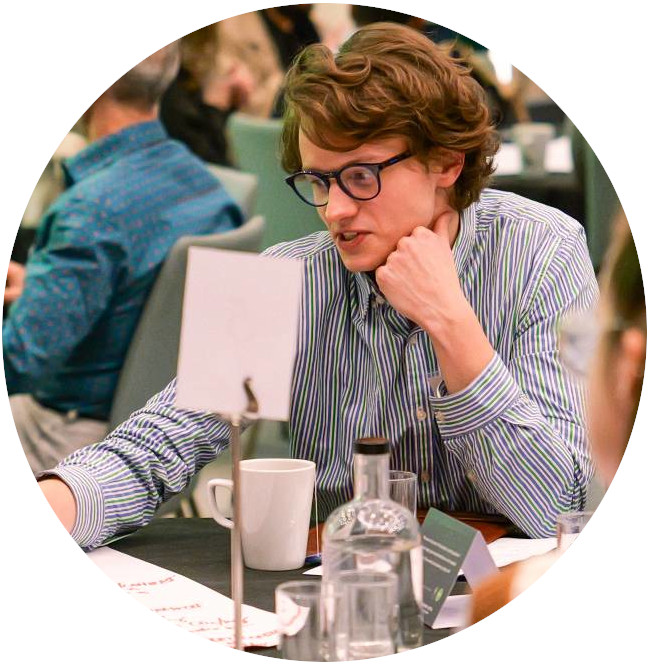
\includegraphics[width=5cm]{p1000137-cropped.jpg}
\vspace{-0.3cm}
\section{Contact}
\vspace{0.1cm}Mobile: \texttt{+447719679958}
~
Email: \texttt{rossgardiner24@gmail.com}
~
GitHub: \url{https://github.com/rossGardiner}
~
LinkedIn: \url{https://www.linkedin.com/in/ross-g/}
~ 
Orcid: \url{https://orcid.org/0000-0001-5633-1317}
%

\section{Programming Languages}
Bash, Python, C++, C, Haskell, Java, C\#, \LaTeX, MATLAB, HTML/CSS, R
%
\section{Recent Technologies}
PyTorch, OpenCV, Tensorflow/Keras, NVIDIA~CUDA, Linux, MS .NET, Qt, Doxygen, Sphinx, Google~Test, Docker
\section{Miscellaneous Skills}
UK Driver's Licence, Video~and~Photo~Editing,
Electronics~Design/Manufacture, Vehicle Repair, Woodwork, Rock Climbing
\vspace{-0.2}
\section{Awards/Recognition}
Year in Industry Contribution to the Business Awards: Scottish Winner (2016),
~
Year in industry IETF Future Industry Leaders Awards: Innovation Prize (2016);
~
Leonardo Employee Recognition Award (2019)
\end{aside}
  \vspace{-0.4cm}

\section{About}
  \vspace{-0.36cm}

Enthusiastic \textbf{MEng Electronics and Software Engineering graduate} embarking on a \textbf{PhD in Artificial Intelligence} at the University of Exeter. I have a keen interest in applications of machine learning and methods in ecological research. I am currently seeking opportunities complementary to my PhD, working with cutting-edge technologies wherein a strong foundation in electronics, software engineering, AI methods and ecological knowledge may be applied.
  \vspace{-0.2cm}
\section{Publications}
  \vspace{-0.3cm}
\begin{entrylist}
\entry
{2025}
{ICCV 2025 (CV4E Workshop) }
{}
{\jobtitle{\href{https://openaccess.thecvf.com/content/ICCV2025W/CV4E/html/Gardiner_Bridging_Domain_Gaps_for_Fine-Grained_Moth_Classification_Through_Expert-Informed_Adaptation_ICCVW_2025_paper.html}{Bridging Domain Gaps for Fine-Grained Moth Classification Through Expert-Informed Adaptation and Foundation Model Priors}} \\ Advances insect camera trap AI through foundation models, expert knowledge and compression with knowledge distillation.}
\entry
{2025}
{Methods in Ecology and Evolution: AI for Conservation special feature}
{}
{\jobtitle{\href{https://besjournals.onlinelibrary.wiley.com/doi/10.1111/2041-210X.70098}{Towards Scalable Insect Monitoring: Ultra-Lightweight CNNs as On-Device Triggers for Insect Camera Traps}} \\ Develops efficient and explainable AI, quantised for microcontroller deployment, to enable scalable insect monitoring. }
  \entry
    {2022}
    {Ecological Informatics Journal}
    {}
    {\jobtitle{\href{https://doi.org/10.1016/j.ecoinf.2022.101657}{Motion vectors and deep neural networks for video camera traps}}\\ Contributes to advancements in animal detection in challenging environments via divergence from traditional PIR sensors.}
    \end{entrylist}
  \vspace{-0.2cm}
\section{Employment History}
  \vspace{-0.3cm}
  
\begin{entrylist}
\entry
{\scalebox{.8}[1.0]{September 2023 -- Present}}
  {University of Exeter}
  {University of Exeter}
  {\jobtitle{Postgraduate (PhD) Researcher and Teaching assistant}\\
  My research is focused on the development of AI technologies for biodiversity monitoring. I am particularly interested in: how large-scale self-supervised foundation models can be leveraged for rapid ecological assessment, how explainable-AI techniques can be explored to build trust in learned representations from fine-grained and long-tailed training datasets and how AI can operate at the edge in conjunction with growing specialised conservation hardware solutions. I concurrently work as a Teaching Assistant.
  }
%\entry
%  {\scalebox{.8}[1.0]{March 2023 -- August 2023}}
%  {Freelance Work}
%  {Remote and On-site}
 % {\jobtitle{Electronic Engineer}\\
%  Delivered comprehensive electronic engineering solutions over two projects for a small renewables business in Lerwick, Shetland. Both projects included the delivery of charge controllers designed by myself, this included electronic circuit design and specification of components, layout planning, and board manufacturing/assembly. Additionally, I engineered robust event-driven firmware for Microchip PIC devices for the programmable aspects of my designs. 
%  }
\entry
  {\scalebox{.8}[1.0]{June 2021--March 2023}}
  {DynAikon Ltd.}
  {Entirely Online}
  {\jobtitle{Software Developer \& Research Assistant}\\
  I worked primarily as the project lead for our software package, \linkrg{https://dynaikon.com/trap/}{DynAikonTrap}. This is a fully open-source camera trap with some AI capability and integration with our \linkrg{https://service.fastcat-cloud.org/api/spec}{web API} for observation logging. This is a novel design, using video encoding artefacts and convolutional neural networks to detect animal presence in a live video feed. Aspects are discussed in our \linkrg{https://www.sciencedirect.com/science/article/pii/S1574954122001066}{paper}. 
  \\
  As project lead I have been involved in every aspect of software development, communication, product support and liaison with our funding consortium. I also produced my final-year MEng \linkrg{https://gitlab.dynaikon.com/rossg/2190583_Gardiner_ENG5041P_Final_Year_Report/}{research project} from work completed on DynAikonTrap: successfully halving the system power consumption, accelerating our CNN detectors via weight quantisation and adding capability to distinguish humans from animals in video feed. 
  %Recently, I have been preparing for a workshop where I  introduce DynAikonTrap to a group of wildlife researchers at the Spanish National Research Council in Catalonia. We hope this will help the project gain traction and volunteers for the open source development effort.
  %\\
  %\textbf{Technologies currently in use: }
  %\begin{itemize}
  %  \item \textbf{Python} programming language is used throughout while \textbf{Cython} is used for some real-time video processing aspects. \textbf{C/C++} is used for our video decoding library. 
  %  \item \textbf{Sphinx} handles our automated documentation generation. A \textbf{GitLab CI-runner} compiles and publishes docs to our website via a \textbf{Docker} container. 
   % \item Deep learning and computer vision capabilities are provided through the \textbf{OpenCV} library and \textbf{TFLite} runtime. Model training has been undertaken using the \textbf{Tensorflow} object detection API.
   % \item As a hardware platform, we use the \textbf{Raspberry Pi} system and we package our software for compatibility with \textbf{Ubuntu/Linux} systems.
    
%\end{itemize}
}
%------------------------------------------ ------
\entry
  {\scalebox{.8}[1.0]{June--Sept.  2020}}
  {Imagination Technologies}
  {Kings Langley, Watford}
  {\jobtitle{Vision \& AI Research Intern}\\
As a Research Intern on the Compiler Team, I analysed image metrics to assess neural network quality, specifically for GANs. I developed a \textbf{Python}-based evaluative test for a \textbf{Jenkins} server, integrating it into the compiler's fault-checking pipeline. My responsibilities included Agile collaboration, participating in stand-ups, and producing detailed reports on metrics.
 }
\entry
  {\scalebox{.8}[1.0]{Aug. 2018--June 2019}}
  {Leonardo UK Ltd.}
  {Crewe Road, Edinburgh}
  {\jobtitle{Undergrad Placement Engineer (Systems Dept.)}\\
  In my university gap year at Leonardo, I focused on radar simulation product development, managing quarterly software releases and implementing algorithms with real-time GPU processing using NVIDIA CUDA API. I successfully mastered new technologies, contributing to hardware acceleration improvements. My work culminated in a well-received report on these advancements and their integration into existing products.
}
\entry
  {\scalebox{.8}[1.0]{June--Sept. 2017}}
  {Leonardo UK Ltd.}
  {Crewe Road, Edinburgh}
  {\jobtitle{Summer Placement Engineer (Systems Dept.)}\\
  I enhanced my radar imaging simulation project, achieving a tenfold increase in simulation speed by implementing hardware acceleration with \textbf{C#/.NET} and NVIDIA \textbf{CUDA C}. My role included conducting weekly progress meetings, documentation in a lab book, and presenting results, which enabled simulations to complete in a lunch break instead of overnight.
}
\entry
  {\scalebox{.8}[1.0]{August 2015 --July.  2016}}
  {Leonardo UK Ltd.}
  {Crewe Road, Edinburgh}
  {\jobtitle{Year in Industry Student (Systems Dept.)}\\
 Selected for Leonardo's Systems Engineering Year in Industry program straight from high school, I developed software to simulate specialised synthetic aperture radar ground imaging. This involved creating a "virtual" flight trial using digital terrain from freely available map data. The transition required significant adaptation; I completed a five-day company radar course, learned to develop robust \textbf{C#/.NET} software to company standards, and built resilience and self-awareness. My contributions earned multiple Year in Industry awards and led to an invitation to return the following summer.
}


%------------------------------------------------
\end{entrylist}
\hspace*{-5.5cm}\begin{minipage}[b]{1.4\textwidth}
%\vspace{-0.6cm}
\section{Education}
  \vspace{0.2cm}
\begin{entrylist}
%------------------------------------------------
\entry
{\scalebox{.8}[1.0]{Sept. 2016--June 2022}}
{MEng, Electronic and Software Engineering}
{University of Glasgow}
{
I graduated from the James-Watt School of Engineering \textbf{with Honours of the First Class}. My degree includes a practical mix of electronic design with computing science theory and application.
I have enjoyed working on team projects throughout my studies. For two such projects in my final year, I took on the role of lead programmer. This involved managing our team's overall direction and ownership of event-driven software in \textbf{C/C++} . As part of GUSTS - Glasgow University Sustainable Technology Society I served as Projects Manager in the 2020-2021 committee group and helped organise events promoting sustainable engineering projects on campus. I've also been a keen member of the University Surf Club, which has been a lot of fun. Finally, I enjoyed serving as a lab demonstrator for a \textbf{Python} web app development course, where I learned teaching methods and solidified my own knowledge.
\vspace{0.1cm}


%\entry{}{\hspace*{-2.3cm}Selected Achieved Grades}{}{

Selected achieved grades tabulated below; achieved an \textbf{overall GPA of 18.6/22.0}:

\vspace{0.2cm}

\centering
\begin{tabular}{L{4.9cm}C{1cm}C{1cm} C{0.0cm}L{4.6cm}C{1cm}C{1cm}}
\toprule
\textbf{Course} & \textbf{Grade} & \textbf{Year} & & \textbf{Course} & \textbf{Grade} & \textbf{Year}\\ \midrule
 \linkrg{https://www.gla.ac.uk/coursecatalogue/course/?code=ENG5041P}{Individual Project (Final Year)}             & A2         & 5\textsuperscript{th}       & & \linkrg{https://www.gla.ac.uk/coursecatalogue/course/?code=ENG4053}{Digital Signal Processing}  & A3             & 4\textsuperscript{th}  \\ \midrule
 \linkrg{https://www.gla.ac.uk/coursecatalogue/course/?code=ENG5220}{Real-time Embedded Programming}            & A2         & 5\textsuperscript{th}       & & \linkrg{https://www.gla.ac.uk/coursecatalogue/course/?code=ENG4173}{Renewable \& Sustainable Energy}        & A4             & 4\textsuperscript{th}\\ \midrule
 \linkrg{https://www.gla.ac.uk/coursecatalogue/course/?code=ENG5026}{Design Special Topic}             & A4         & 5\textsuperscript{th}       & & \linkrg{https://www.gla.ac.uk/coursecatalogue/course/?code=UESTC3020}{Digital Circuit Design} & A1 & 3\textsuperscript{rd} \\ \midrule
 \linkrg{https://www.gla.ac.uk/coursecatalogue/course/?code=COMPSCI4021}{Functional Programming}             & A2             & 4\textsuperscript{th}         & & \linkrg{https://www.gla.ac.uk/coursecatalogue/course/?code=UESTC3003}{Electronic System Design} & A2 & 3\textsuperscript{rd}\\ \bottomrule
\end{tabular}

}
\vspace{0.2cm}


\entry
{\scalebox{.8}[1.0]{2014--2016}}
{Open University Modules}
{Open University (Online)}
{Throughout my final year of high-school and my Year in Industry placement, I studied remotely for  \linkrg{https://www.open.ac.uk/courses/modules/m250}{M250 - Object-oriented Java programming} and \linkrg{https://www.open.ac.uk/courses/modules/m269}{M269 - Algorithmns, data structures and computability}, achieving a Pass grade for both. These modules have served as my first qualification in the computing/software engineering world and helped fuel my early interest in the subject.   }
%------------------------------------------------

%\entry
%{\scalebox{.8}[1.0]{2015--2016}}
%{First-line Management Diploma}
%{Perth College UHI}
%{As a student on the Year-in-industry programme, I was invited to enrol in a \linkrg{https://www.perth.uhi.ac.uk/courses/chartered-management-institute-first-line-management}{a level 6 management diploma} at Perth College. This taught fundamentals of business etiquette, teamworking skills via a selection of assignments delivered via online learning. I achieved a Pass grade along side my work at Leonardo UK Ltd..}
%------------------------------------------------
\vspace{0.2cm}

\entry
{\scalebox{.8}[1.0]{2010--2015}}
{Peebles High School}
{Springwood Rd, Peebles}
%------------------------------------------------

\end{entrylist}
\end{minipage}

\hspace*{-5.5cm}\begin{minipage}[b]{1.4\textwidth}
\vspace{-0.4cm}
\section{Open-Sourced Software Projects}
  \vspace{0.1cm}
I am passionate about open sourced software. Many of my own contributions to software in the public domain are available on my personal GitHub site and through DynAikon's public git repository. Below are some example projects I am proud of.
\vspace{0.1cm}
\begin{entrylist}
\entry
{June 2021--Present}
{DynAikonTrap - AI Camera Trap for Biodiversity Monitoring}
{Python/C}
{
Codebase: \linkrg{https://gitlab.dynaikon.com/dynaikontrap}{\texttt{gitlab.dynaikon.com/dynaikontrap}} Our published paper: \linkrg{https://doi.org/10.1016/j.ecoinf.2022.101657}{\texttt{doi.org/10.1016/j.ecoinf.2022.101657}}\\
Documentation: \linkrg{https://dynaikon.com/trap-docs/}{\texttt{dynaikon.com/trap-docs/}} \\My final-year dissertation: \linkrg{https://gitlab.dynaikon.com/rossg/2190583_Gardiner_ENG5041P_Final_Year_Report/}{\texttt{gitlab.dynaikon.com/rossg/2190583\_Gardiner\_ENG5041P\_Final\_Year\_Report/}}
}
\vspace{0.1cm}
\entry
{Jan.--May 2022}
{Signapse - AI Sign Language Teacher}
{C++/C}
{
A simple event-driven video processing app using a convolutional image classifier to teach hand signs via a user interface. \\
Codebase: \linkrg{https://github.com/albanjoseph/Signapse}{\texttt{github.com/albanjoseph/Signapse}} Wiki: \linkrg{https://github.com/albanjoseph/Signapse/wiki}{\texttt{github.com/albanjoseph/Signapse/wiki}} \\
Documentation: \linkrg{https://albanjoseph.github.io/Signapse/html/annotated.html}{\texttt{albanjoseph.github.io/Signapse}}
}
\vspace{0.1cm}
\entry
{Jan.--May 2022}
{AudiClean - Event-driven Audio Filtering Library}
{C++/C}
{
Extension of the SoX audio library, provides implementation of novel audio filtering mechanisms and a command-line interface.\\
Codebase: \linkrg{https://github.com/rossGardiner/AudiClean}{\texttt{github.com/rossGardiner/AudiClean}} Documentation: \linkrg{https://rossgardiner.github.io/AudiClean/html/annotated.html}{\texttt{rossgardiner.github.io/AudiClean}}
} 
\vspace{0.1cm}
\entry
{Sept. 2019--May 2020}
{NextSteps - Sports-ground Test Equipment Driver}
{Java}
{
Codebase: \linkrg{https://github.com/rossGardiner/next-steps}{\texttt{github.com/rossGardiner/next-steps}}


}
%------------------------------------------------
\end{entrylist}
  \vspace{0.2cm}
%----------------------------------------------------------------------------------------
% INTERESTS SECTION
%----------------------------------------------------------------------------------------3
\end{minipage}
%\vspace{0.0}\hspace*{-5.5cm}\begin{minipage}[b]{1.4\textwidth}
%\section{Personal Interests}
%  \vspace{0.05cm}
%In my free time I am keen on exploring the great outdoors. My favourite past-times are \textbf{camping, climbing and surfing} when I get the chance. During time off, you can find me exploring the west coast with my girlfriend in our camper van and throughout much of this summer I have been enjoying Scotland's diverse range of \textbf{rock climbing} venues. I also love training for climbing and bouldering in my local gym and take a keen interest in fitness and nutrition.

%\end{minipage}
%----------------------------------------------------------------------------------------

%\vspace{-0.1cm}\hspace{1cm}\begin{minipage}[b]{\textwidth}
%\hline
%\vspace{0.05cm}
%\footnotesize{
%How's my work? I'd be thrilled to receive any feedback on my CV you may have: \linkrg{https://tbana5tiy5p.typeform.com/to/LwEMHwuO}{complete my survey}.\\
%This CV has been created and edited using \LaTeX, the style sheet used is provided under GPLv3 on \linkrg{https://github.com/rossGardiner/RossGardiner-CV}{my GitHub}.}
%\end{minipage}
%\blfootnote{How's my work? I'd be thrilled to receive any feedback on my CV you may have: \linkrg{https://tbana5tiy5p.typeform.com/to/LwEMHwuO}{complete my survey}.}
%\blfootnote{This CV has been created and edited using \LaTeX, the style sheet used is provided under GPLv3 on \linkrg{https://github.com/rossGardiner/RossGardiner-CV}{my GitHub}.}
\end{document}